%
% File emnlp2015.tex
%
% Contact: daniele.pighin@gmail.com
%%
%% Based on the style files for ACL-2015, which were, in turn,
%% Based on the style files for ACL-2014, which were, in turn,
%% Based on the style files for ACL-2013, which were, in turn,
%% Based on the style files for ACL-2012, which were, in turn,
%% based on the style files for ACL-2011, which were, in turn, 
%% based on the style files for ACL-2010, which were, in turn, 
%% based on the style files for ACL-IJCNLP-2009, which were, in turn,
%% based on the style files for EACL-2009 and IJCNLP-2008...

%% Based on the style files for EACL 2006 by 
%%e.agirre@ehu.es or Sergi.Balari@uab.es
%% and that of ACL 08 by Joakim Nivre and Noah Smith

\documentclass[11pt,a4paper]{article}
\usepackage{acl2015}
\usepackage{times}
\usepackage{url}
\usepackage{latexsym}
\usepackage{graphicx,subfigure}
\usepackage{devanagari}
\usepackage{amsmath}
\usepackage{multirow}
\usepackage{float}

%\setlength\titlebox{5cm}

% You can expand the titlebox if you need extra space
% to show all the authors. Please do not make the titlebox
% smaller than 5cm (the original size); we will check this
% in the camera-ready version and ask you to change it back.


\title{Words are not Equal: A Graded Weighting Model for improving Additive Composition of Word Vectors}

\author{Pranjal Singh \\
  Dept. of Computer Science \& Engg. \\
  IIT Kanpur \\
  {\tt spranjal@iitk.ac.in} \\\And
  Amitabha Mukerjee \\
  Dept. of Computer Science \& Engg. \\
  IIT Kanpur \\
  {\tt amit@cse.iitk.ac.in} \\}
\date{}

\begin{document}
\maketitle
\begin{abstract}
In recent years, distributional semantics and neural language models for words and documents have been proposed to perform various NLP tasks ignoring earlier models such as tf-idf. Since both word vector model and document vector models are built separately, there combined efficacy as well as using word vectors to build document vectors have been ignored. We propose a graded weighting scheme for building document vectors which can be combined with document vectors trained separately as well as tf-idf representation used earlier to achieve state-of-the art results in sentiment classification on classical IMDB movie review dataset achieving an accuracy of 94.19\%(improvement of 1.61\% over previous best). We also implement an ensemble model which boosts our accuracy by about 0.5\% using recursive neural network. Since these are language free models and can be obtained in an unsupervised manner, they are of interest for under-resourced languages such as Hindi as well and many more languages. We demonstrate the language free aspects by developing a huge increment on results for Hindi with an impressive accuracy gain on state of the art by 12\% (from 80\%) for two review datasets.
\end{abstract}

\section{Introduction}
Language representation is a very crucial aspect to perform various NLP tasks and has been looked into great detail in recent times. Languag representation models have fallen into broadly two categories: ones which are language dependent models(e.g.,\cite{Socher:13}) and ones which are language independent models(e.g., LDA, BOW, SkipGram, NLM, etc.). 

Language independent models such as LDA  and BOW have been quite effective since long time. Variants of BOW such as tf-idf had changed the perception of researchers towards these models when they were proved effective in various NLP tasks. LDA was able to model inter and intra documental statistical and relational structure quite well overcoming the drawbacks of BOW. But the semantic and syntactical dependencies were still ignored. After the introduction of neural language vector models, NLP saw a huge diversion in representation of words and documents.

For individual words, vectors are obtained via distributional learning, the mechanisms for which varies from document-term matrix factorization~\cite{Landauer:97}, various forms of deep learning~\cite{Collobert:08,Turian:10,Socher:13}, optimizing models to explain co-occurrence constraints ~\cite{Mikolov:13a,Pennington:14},etc. Once the word vectors have been assigned, similarity between words can be captured via cosine distances. The same models have been extended(\cite{Le:14}) with new variables to build vector models for sentences and documents. These models include the essence of individual words as well as their relative order in terms of sentence vector which was earlier absent in word vectors. The advantage of these approaches is that they can capture both the syntactic and the semantic similarity between words/documents in terms of their projections onto a high-dimensional vector space; further, it seems that one can tune the privileging of syntax over semantics by using local as opposed to large contexts~\cite{Huang:12}.

Some grammarians have been trying to find whether sentence meaning accrues by combining word meanings, or whether words gain their meanings based on the context they appear in \cite{Matilal:90}. We develop on this idea and propose a graded weighting scheme to build document vectors from word vectors. This idea is merged with obtaining document vectors separately in the form of distributed learning as well as tf-idf. This combined model is language independent and is enriched with vital properties of other models. This ensures that our model is effective as well as accurate in various languages. 
We then go a step ahead to build an ensemble of our model and recurrent neural network, which essentially has the properties of a generative model, to achieve state-of-the-art result on IMDB movie review dataset(94.19\%) with a significant improvement over previous best.
The world class results in English clearly indicate the efficacy of our approach and improvements in Hindi depict the deficiency in other models which were used earlier.
\section{Related Work}

\subsection{Sentiment Analysis}
In order to evaluate the efficacy of the model, we apply it to the task of sentiment analysis. Here the problem is that of identifying the polarity of sentences (Liu et al. 2012); for example: 
\begin{itemize}
\item Positive: {\dn rA\8{m} n\? khAnF kF r\327wtAr khF{\qva} Tmn\? nhF{\qva} dF} [Ramu didn't allow the pace of the story to subside]
\item Negative: {\dn pd\?{\qvb} pr EdKAyA jA rhA KO\327w Esn\?mAGr m\?
nhF{\qva} psr pAtA} [The horror shown on the screen didn't reach the theater]
\end{itemize}
Majority of the existing work in this field is in English (Pang and Lee, 2008). \cite{Sharma:14} give a summary of work done in Hindi in the field of opinion mining.
This is a problem that has attracted reasonable attention in both Hindi and English (see section~\ref{sec:related}). There have been heuristic based and machine larning based models used in this domain~\cite{Wang:14}. Heuristic based methods, in general, classify text sentiments on the basis of total number of derived positive or negative sentiment oriented features. For example, Hatzivassiloglou and McKeown \cite{Hatzivassiloglou:97} described that adjectives are more predictive of sentiment classification and they predicted the sentiment of adjectives by inspecting them in conjunction with "and", "or", "but", "either/or" and "neither/nor". However the problem with this approach is that even if adjectives  are important in many languages but this model underestimates some predictive words of other parts-of-speech which may be important in some languages. Also these models rely heavily on human engineered features which, in general, is a domain and language dependent task.
\cite{Mikolov:10} claim that size of hidden layer reflects amount of training data with smaller size leading to less number of layers. Weights are initialized to random small values and updated using gradient descent.
\cite{Mikolov:11} present several modifications of the original recurrent neural network language model (RNN LM). The present approaches that lead to more than 15 times speedup for both training and testing phases. They also show the importance of backpropagation through time(BPTT) which is an extension to backpropagation algorithm for recurrent networks. With truncated BPTT, the error is propagated through recurrent connections back in time for a specific number of time steps. Thus, the network learns to remember information for several time steps in the hidden layer when it is learned by the BPTT.

Sentiment analysis is a well-known research area in NLP today (see reviews in~\cite{Liu:12} and Pang et al. (2008), and also
challenge in SemEval-2014).  Early work on movie review sentiments achieved an accuracy of 87.2\% (Pang et al. 2004) on a dataset that discarded objective sentences and used text categorization techniques
on the subjective sentences. Le and Mikolov (2014) use word vector models and obtain 92.6\% accuracy on IMDB movie review dataset.
They used distributed bag-of-words model, which they call as \emph{paragraph vector}. More difficult challenges involve short texts with nonstandard vocabularies,as in twitter.  Here, some authors focus on building extensive feature sets (e.g. Mohammad et al.(2013); F-score 89.14). \\
% WANG IS NOT BEING REFERRED TO
Wang et al. (2014) propose a word vector neural-network model, which takes both sentiment and semantic information into account. This word vector expression model learns word semantics and sentiment at the same time as well as fuses unsupervised contextual information and sentence level supervised labels.

Neelakantan et al.(2015)\cite{Neelakantan:14} took word vector models to next level where they proposed multiple embeddings per word. Nearly all the work before this assumes a single vector per word
type—ignoring polysemy and thus jeopardizing their usefulness for downstream tasks. The authors present an extension to the Skip-gram model that efficiently learns multiple embeddings per word type. It differs from recent related work by jointly performing word sense discrimination and embedding learning, by non-parametrically estimating the number of senses per word type, and by its efficiency and scalability. They achieve state-of-the-art results in the word similarity in context task and demonstrate its scalability by training with one machine on a corpus of nearly 1 billion tokens in less than 6 hours.

Since most sentiment analysis is oriented towards semantics, and one may bypass the syntactic
processing which remains poor for Hindi. Methods that have been used are largely based on assigning a sentiment effect for individual words, and then combining these in some manner to come up with an overall sentiment for the document. Such methods ignore word order and have been criticized since the import of a sentence can change completely simply by re-arranging the words, though the sentiment evaluation remains the same. Several groups have attempted to improve the situation by modeling the composition of words into larger contexts \cite{Le:14,Socher:13,Johnson:14,Baroni:14}.

However, most of the work on sentiment analysis in Hindi has not attempted to form richer compositional analyses.   For the type of corpora used here, the best results, obtained by combining a sentiment lexicon with hand-crafted rules (e.g. modeling negation and "but" phrases), reach an accuracy of 80\%~\cite{Mittal:13}.

There has been limited work on sentiment analysis in Hindi -- see review in
~\cite{Medagoda:13}, who surveys sentiment analysis in non-English languages). Joshi et al. (2010) compared three approaches: In-language sentiment
analysis, Machine Translation and Resource Based Sentiment Analysis. By using WordNet linking, words in English SentiWordNet were replaced by equivalent Hindi words to get H-SWN. The final accuracy achieved by them is 78.1\%.

\cite{Bakliwal:12}
traversed the WordNet ontology to antonyms and synonyms 
to identify polarity shifts in the word space. Further
improvements were achieved by using a partial stemmer (there is no good
stemmer / morphological analyzer for Hindi), and focusing on 
adjective/adverbs (45 + 75 seed words given to the system); their 
final accuracy was 79.0\% for the product review dataset. 
Mukherjee et al. (2012) presented the inclusion of discourse markers in a bag-of-words model and how it improved the sentiment classification accuracy by 2-4\%.  % <--- NOT HINDI
Mittal et al. (2013) incorporate hand-coded rules dealing with negation and discourse relations and extend the HSWN lexicon with more opinion words.  Their algorithm achieves  80.2\%
accuracy on classification of movie reviews on a separate dataset.\\

\cite{Mikolov:10} presents new recurrent neural network based langauge model which has found vital application in various NLP tasks as well. They provide ample empirical evidence to suggest that connectionist language models are superior to standard n-gram techniques, except their high computational (training) complexity. The model has also been extended to speedup training time by few optimizations.(More details in \ref{sec:rnn}).

For resource-poor languages, these approaches have the added lure that many of these methods are completely unsupervised and work directly with large raw text corpora, thus avoiding contentious issues such as deciding on a POS-tagset, or expensive human annotated resources such as treebanks.  For Indian languages which are highly inflected, stemming or identifying the lemma is another problem
which such models can overcome, provided the corpus is large enough. Nonetheless, this approach remains under-explored for Indian languages. At the same time, it must be noted that many approaches seek to improve their performance by combining POS-tags and even parse tree structures into the models for higher accuracies in specific tasks~\cite{Socher:13}.  One problem in this approach is that of  combining the word vectors into larger phrases. In past work, inverse-similarity weighted averaging appears to work to some extent even for complex tasks such as essay grading \cite{Landauer:03}, but multiplicative models (based on a reducing the tensor products of the vectors) appears to correlate better with human judgements~\cite{Mitchell:08,Socher:13}.
Another complexity in composition is that composing words across phrasal boundaries are less meaningful than composing them within a phrase - this has led to models that evaluate the nodes of a parse tree, so that only coherent phrases are evaluated~\cite{Socher:13}. The results reported here, are based on applying the Skip-Gram  model~\cite{Mikolov:13b} to Hindi.\\
\cite{Turney:10} give a detailed overview of various vector space models and their composition. A surprising event in Information Theory has higher information content than an expected event (Shanon, 1948). The same happens when we give weights to word vectors. We give more weights to events which occur by surprise and less weight to events which are expected. The most popular weighting concept in this domain is the idea of tf-idf which is explained later. \cite{Salton:88} defined a large family of tf-idf weighting functions and evaluated them on information retrieval tasks, demonstrating that tf-idf weighting can yield significant improvements over raw frequency. Term weighting is also significant in reducing the weights of highly correlated words such as \emph{hostage} and \emph{hostages} when they occur together (Church, 1995). \cite{Chirawichitchai:14} have found use of term weighting in sentiment classification in Thai language.

Our model uses concatenation of average word vectors, sentence vectors and tf-idf to build informative document vectors which constitute a feature set for our SVM classier. We have used skip-gram model (Mikolov et al., 2013b) for building word vectors because deep network model of Collobert et al.(2008) takes too much time for training. Also the word embeddings obtained by them are not as good as those obtained by Mikolov et al.(2013b). The main advantage of using skip-gram is that it is computationally less expensive than other neural language models with a complexity of O(log V) instead of O(V). They use hierarchical softmax(\cite{Morin:05}) to achieve such computational efficiency.


\section{Method}
The algorithms and data structures used in this thesis have been introduced and discussed below.
\label{sec:skipgram}
Mikolov et al. (2013b) proposed two neural network models for building word vectors from large unlabeled corpora; Continuous Bag of Words(CBOW) and Skip-Gram.  In the CBOW model, the context is the input, and one tries to learn a vector for the central word; in Skip grams, the input is the target word and one tries to guess the set of contexts.  The Skip gram was found to perform better on smaller corpora, and here we have focused on this model for building our word vectors. The model uses each current word as an input to a log-linear classifier with continuous projection layer, and predict words within a certain range before and after the current word. The objective is to maximize the probability of the context given a word within a language model:

\begin{center} $p(c|w;\theta)=\frac{\exp^{v_c.v_w}}{\sum_{c' \in C}\exp^{v_c.v_w}}$ \end{center}
where $v_c$ and $v_w$ $\in$ $R^d$ are vector representations for context $c$ and word $w$ respectively. $C$ is the set of all available contexts. The parameters $\theta$ are $v_ci$, $v_wi$ for $w \in V$, $c \in C$, $i \in 1,....,d$ (a total of $|C| \times |V| \times d$ parameters).\\


\subsection{tf-idf}
\label{subsec:tfidf}
Let $D=d_1, d_2, d_3....d_N$ be $N$ documents under study and $T=t_1, t_2, t_3,....t_M$ be the $M$ unique terms in these documents, then each document can be represented as a $M$-dimensional vector:\\
$t_d=\{tf_1,tf_2,tf_3,...tf_M\}$\\
$tf-idf$ weights discounts the frequency of terms based on their importance to a particular document in the entire document set collection under consideration. This is done as follows:
\begin{center}
$tfidf(d,t)=tf(d,t) \times \log(\frac{|D|}{df(t)})$ 
\end{center}
Here $df(t)$ is the number of documents in which term $t$ appears.

\subsection{Vector Averaging for phrases}
\label{sec:vectoraveraging}
As an output of the word vector learning, we now have a $n$-dimensional
vector representation for each word in the Hindi corpus.  Now we need to
assign features for sentences and paragraphs taken from the sentiment dataset
(training and test).  Mikolov et al. (2013b) and Levy et al. (2014) show that
many relational similarities can be recovered by means of vector arithmetic
in the embedded space.  Thus, additive models are useful, though
others have claimed that multiplicative models correlate better with human
judgments~\cite{Mitchell:08,Socher:13}.  In this work, we have retained teh
simplicity of vector averaging to model larger chunks of  discourse.
This models the sentence/document in the same high dimensional space.

\subsection{Document Vectors}
This distributed representation of sentences and documents~\cite{Le:14} modifies word2vec (Skip-Gram) algorithm to unsupervised learning of continuous representations for larger blocks of text, such as sentences, paragraphs or entire documents. The algorithm represents each document by a dense vector which is later trained and tuned to predict words in the sentence\/document.\\
In Paragraph Vector framework, every paragraph is mapped to a unique vector and id, represented by a matrix $D$, which is a column matrix. Every word is mapped to a unique vector and word vectors are concatenated or averaged to predict the context, i.e., the next word.\\
The change in this framework is that the $h$(in Skip-Gram model's equation) is now constructed in a different way. It is now constructed using both $W$ and $D$.\\
The contexts are fixed-length and sampled from a sliding window over the paragraph. The paragraph vector is shared across all contexts generated from the same paragraph but not across paragraphs.  The word vector matrix W, however, is shared across paragraphs. i.e., the vector for "good" is the same for all paragraphs.\\

The paragraph vectors and word vectors are trained using stochastic gradient descent and the gradient is obtained via backpropagation.  At every step of stochastic gradient descent, one can sample a fixed-length context from a random paragraph, compute the error gradient from the network in Figure \ref{fig:doc2vec} and use the gradient to update the parameters in our model. At prediction time, one needs to perform an inference step to compute the paragraph vector for a new paragraph. This is also obtained by gradient descent.  In this step, the parameters for the rest of the model, the word vectors W
and the softmax weights, are fixed.

The paragraph vector represents the missing information from the current context and can act as a memory of the topic of the paragraph.

The advantage of using paragraph vectors is that they inherit the property of word vectors, i.e., the semantics of the words. In addition, they also take into consideration a small context around each word which is in close resemblance to the n-gram model with a large n. This property is crucial because the n-gram model preserves a lot of information of the sentence/paragraph, which includes the word order also. This model also performs better than the Bag-of-Words model which would create a very high-dimensional representation that has very poor generalization.


\subsection{Semantic Composition}
\label{sec:composition}
The Principle of Compositionality is that meaning of a complex expression is determined by the meaning of its parts or constituents and the rules which guide this combination. It is also known as \emph{Frege's Principle}. In our case, the constituents are word vectors and the expression in hand is the sentence/document vector. For example,
\begin{center}
\emph{The movie is funny and the screenplay is good}
\end{center}
In the above sentence, consider the word vectors are represented by $w(x)$ and the sentence vector as $S(x)$.

\begin {table}[h!]
\centering
\begin{tabular}{ |c|c| }
\hline
Composition & Accuracy \\ \hline \hline
Average & 88.42 \\ \hline
Weighted Average & 88.41 \\ \hline
Multiplication & 50.30 \\ \hline
\end{tabular}
\caption {Results of Vector Composition with different Operations}
\label{table:composition}
\end{table}
Analyzing the results from Table \ref{table:composition}, we observed that when we deal with large number of features, there is a presence of large number of \emph{zeros} and presence of a single zero in a feature will make that features contribution zero in the final vector, which happens in our case and thus multiplicative composition fails.\\
We, therefore, adopt both simple and weighted average methods in our work. The advantage with addition is that, it doesnot increase the dimension of the vector and captures high level semantics with ease. In fact, \cite{Zou:13} have used simple average to construct phrase vectors which they have later used to find phrase level similarity using cosine distance.\\
\cite{Mikolov:13c} showed that relations between words are reflected to a large extent in the offsets between their vector embeddings. They also use additive composition to reflect semantic dependencies.
\begin{center}
\emph{queen - king $\approx$ woman - man}
\end{center}
\cite{Blacoe:12} clearly show that vectors of Neural Language Model and Distributed Model when used with additive composition outperform those with multiplicative composition in Paraphrase Classification task. DM vectors outperform by nearly giving accuracy difference of 6\%. They also perform very well on Phrase similarity tasks.\\
\cite{Socher:13} also present yet another model for semantic composition but that uses a sentiment treebank which is a very costly structure to build and it is task dependent. For under-resourced languages such as Hindi, it would take years to build (for English, task done through Amazon Mechanical Turk). This leads to appreciation of models such as Additive Composition.\\
When an n-gram is given to the compositional models, it is parsed into a binary tree and each leaf node, corresponding to a word, is represented as a vector. Recursive neural models will then  compute parent vectors in a bottom up fashion using different types of compositionality functions $g$. The parent vectors are again given as features to a classifier.

\subsection{Dimensionality Reduction}
\label{sec:dimensionality_reduction}
Dimensionality Reduction is the process of reducing the number of random variables in such a way that the remaining variables effectively reproduce most of the variability of the dataset.
The reason for using such techniques is because of the \emph{curse of dimensionality} which is a phenomena that occurs in high-dimension but doesn't occur in low-dimension.\\

\begin{table}[h!]
\small
\begin{tabular}{|p{3.5cm}|p{1.5cm}|p{1.5cm}|}
\hline
\textbf{Method} & \textbf{Feature Selection} & \textbf{Accuracy} \\ \hline
\multirow{3}{*}{Document Vector}              & None      & 74.57 \\ \cline{2-3} 
                                              & PCA(n=50) & 76.33 \\ \cline{2-3} 
                                              & ANOVA-F & 88.07 \\ \hline
\multirow{3}{*}{Weighted Average Word Vector} & None      & 76.43 \\ \cline{2-3} 
                                              & ANOVA-F   & 90.37 \\ \cline{2-3} 
                                              & PCA(n=50) & 78.61 \\ \hline
\end{tabular}
\caption {Accuracies on 700-Movie Review Dataset}
\label{table:700_movie_features}
\end{table}

Table \ref{table:700_movie_features} summarizes how feature selection has improved classification accuracy on the 700 Movie review dataset. With ANOVA-F, we selected around 4k features but with PCA, this number was just 50. So, the low accuracy with PCA can be attributed to the fact that we may have lost some important features in low dimension. Also, PCA cannot work with size of dimension $d>$\emph{size of learning set}.\\
This sharp decrease in accuracy in both cases: Document vector and Weighted Average word vector happens because ANOVA-F selects features with larger variance across group and thus reduces noise to a larger extent whereas PCA reduces angular variance which is not effective in this case due to the distribution of data points in high-dimensional space.

\section{Experiment}
\label{sec:experiment}
In this section, we describe the experiments and analyze the results.

\subsection{Datasets}
We have used 3 datasets for experiments in Hindi and 5 for English. All the datasets including our self created Hindi dataset are described below.\\
We experimented on two Hindi review datasets. One is the Product Review dataset (LTG, IIIT Hyderabad) containing 350 Positive reviews and 350 Negative reviews. The other is a Movie Review dataset (CFILT, IIT Bombay) containing 127 Positive reviews and 125 Negative reviews. Each review is around 1-2 sentences long and the sentences are mainly focused on sentiment, either positive or negative.\\
Our 700-Movie Review Corpus in Hindi contains movie reviews from websites such as \emph{Dainik Jagran} and \emph{Navbharat Times}. The movie reviews are longer than the previous corpus and contains subjects other than sentiment. There are in total 697 movie reviews from both the websites. The statistics compiled is described below.
\begin {table}[h!]
\centering
\begin{tabular}{ |l|l| }
\hline
\multicolumn{2}{|c|}{\textbf{Overall}} \\
\hline
Positive Reviews & 356 \\ 
Negative Reviews & 341 \\
Total Reviews & 697\\ \hline
\multicolumn{2}{|c|}{29.7 sentences per document} \\ \hline
\multicolumn{2}{|c|}{494.6 words per document} \\
\hline
\end{tabular}
\caption {Statistics of Movie Reviews from Jagran and Navbharat}
\end{table}

For experiments in English, we trained on IMDB movie review dataset (Maas et al.(2013)) which consists of 25,000 positive and 25,000 negative reviews. It also contains an additional 50,000 unlabeled documents for unsupervised learning.

The Trip Advisor Review dataset contains around 240K reviews(206MB) from hotel domain. Reviews with overall rating $>=$3 were annotated as positive and those with overall rating $<$3 were annotated as negative. The dataset was split into 80-20 ratio for training and testing purpose.

We also took amazon reviews for our eperiments. Reviews with overall rating $>=$3 were annotated as positive and those with overall rating $<$3 were annotated as negative. The dataset was split into 80-20 ratio for training and testing purpose. There were 3 review datasets: Watches, Electronics and MP3 each of size 30.8MB, 728.4MB and 27.7MB respectively. Electronics dataset consists of 1,241,778 reviews, Watches Dataset consists of 68,356 reviews and MP3 Dataset consists of 31,000 reviews.

\subsection{SkipGram or CBOW}
SkipGram model tends to predict a context given a word whereas CBOW model predicts a word given a context. It seems intuitive and also from observation~\cite{Mikolov:13b} that SkipGram will perform better on semantic tasks and CBOW on syntactic tasks. We now try to evaluate how they differ on classification accuracies on the two datasets: \emph{Watches} and \emph{MP3}.
\begin{figure}[ht!]
\centering
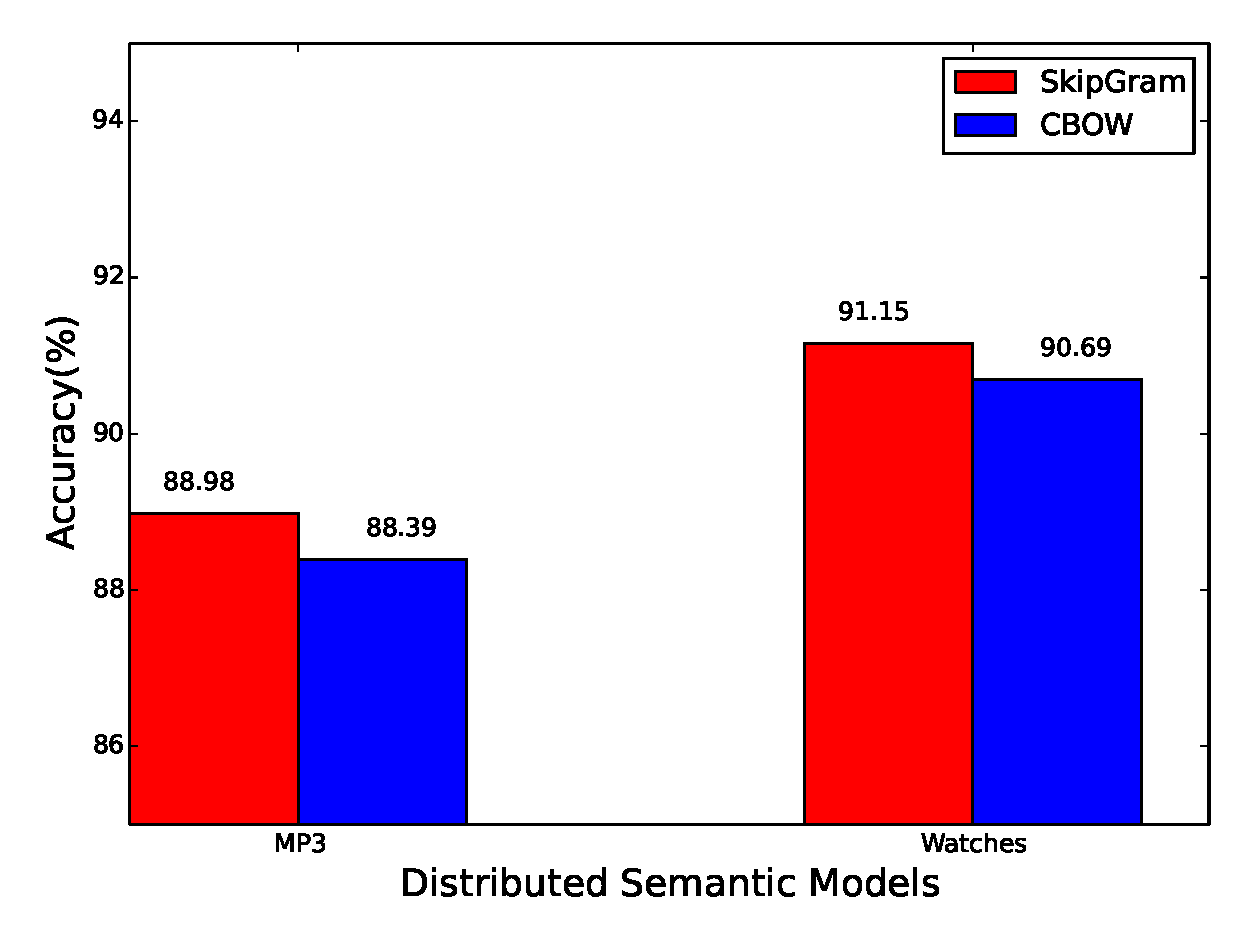
\includegraphics[width=80mm, height=60mm]{img/accuracy_sgcbow.eps}
\caption{Variation of Accuracy with skipgram and cbow on Watches and MP3 Datasets. \label{fig:accuracy_sgcbow}}
\end{figure}
Figure \ref{fig:accuracy_sgcbow} show that skipgram outperforms CBOW on sentiment classification task. It can be justified by the fact that sentiment inclination of a document is more oriented towards semantics of that document rather than just syntax and our results clearly demonstrate this fact.

\subsection{Graded Weighting}
In this experiment, we first generated $n$-dimensional word vectors by training skip-gram model on product and movie review corpus in Hindi and IMDB corpus in English. We then averaged-out word vectors for each document to create document vectors. This now acts as a feature set for that particular document.
We also created \emph{tf-idf} vectors for each document. This can be seen as a vector representation of that particular document. We then concatenated these document vectors with document vectors obtained after averaging-out word vector of each document.

Algorithm \ref{alg:weighted_average} presents a new approach to build document vectors using distributional semantics.Till date, everyone has ignored how to effectively use vector composition techniques and as a result, this area has seen very less attention. But we have successfully used \emph{idf} values to give weights to word vectors and hence obtain much better sentence/document vectors. Refer to \ref{sec:hindi_results} to see how this new technique has improved sentiment classification on Hindi reviews.
The advantage of this model is that once we obtain \emph{idf} values from training corpus, we can directly use it with test corpus without any additional computation.

\subsection{Enhanced Document Vector}
This experiment redefined document representation in NLP used for sentiment classification. It has the property of including both syntactic and semantic properties of a piece of text. The limitations of skip-gram word vectors have been fulfilled by document vectors and hence we achieve state-of-the-art results on IMDB movie review dataset.

This experiment was done on IMDB movie review dataset. Here, we first trained a \emph{recursive neural network} and then obtained predictions on test reviews in terms of probability. We trained another classier(Linear SVM) using Enhanced Document Vectors and then obtained predictions on test reviews. We then merged these two predictions using a simple heuristic to obtain final classification. This led to a tremendous increase in classification accuracy(Refer section \ref{sec:result}).\\

\cite{Maaten:08} represents embeddings
%\begin{figure}[H]
%\centering
%
\includegraphics[width=40mm, height=60mm]{img/tsne.eps}
%\caption{t-SNE visualization of the top 5000 Hindi Words in high dimensional space.  (Magnify to see details). \label{fig:5K_hindi}}
%\end{figure}

%\begin{figure}[]
%\centering
%\begin{subfigure}
%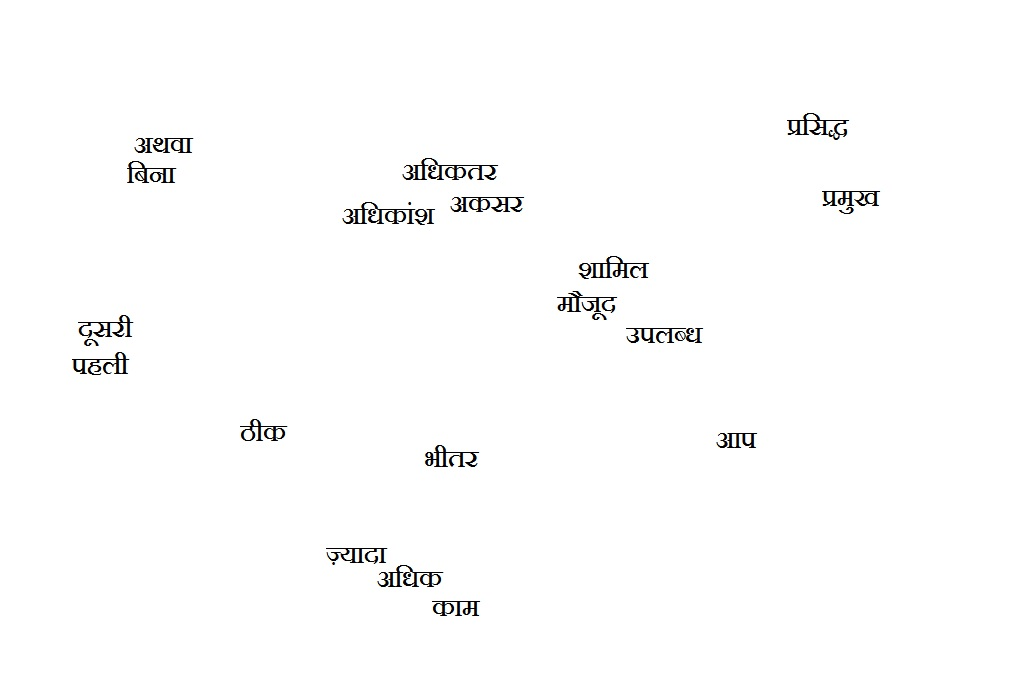
\includegraphics[scale=0.01]{img/5K_hindi_zoom1.eps}
%\caption{}
%\label{fig:5K_hindi_zoom1}
%\end{subfigure}
%\newline
%\begin{subfigure}
%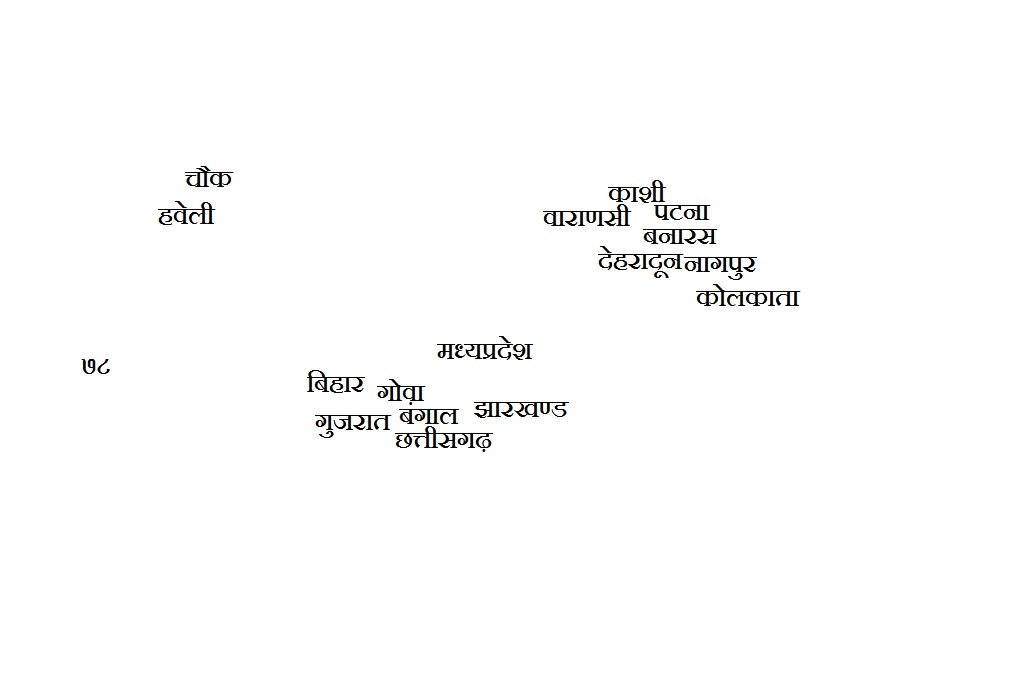
\includegraphics[scale=0.01]{img/5K_hindi_zoom2.eps}
%\caption{}
%\end{subfigure}
%\newline
%\begin{subfigure}
%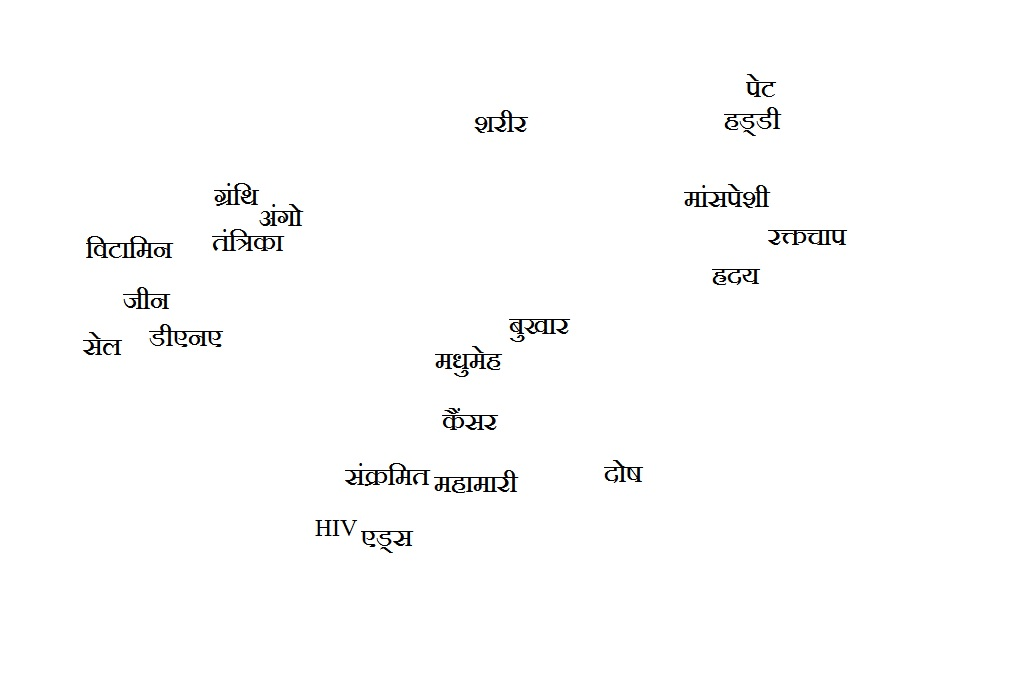
\includegraphics[scale=0.01]{img/5K_hindi_zoom3.eps}
%\caption{}
%\end{subfigure}
%\newline
%\caption{A closer look at two clusters in the visualization showing a) quantity relations, b) locations and c) diseases.}
%\label{fig:5K_hindi_zoom}
%\end{figure}

%Figure \ref{fig:5K_hindi_zoom} gives a closer look into few clusters which depicts the relation between words in high dimensional space. Figure \ref{fig:5K_hindi_zoom1} shows that words such as 
%{\dn mO\8{j}d} and {\dn uplND} are closer to each other but farther from words such as {\dn \31EwyAdA} and {\dn aEDk}.

\subsection{Results}
\begin {table}[H]
\centering
\small
\begin{tabular}{ | c | c | }
\hline
\textbf{Method} & \textbf{Accuracy} \\ \hline
Maas et al.(2011) & 88.89\\ \hline
NBSVM-bi (Wang \& Manning, 2012) & 91.22\\ \hline
NBSVM-uni (Wang \& Manning, 2012) & 88.29\\ \hline
SVM-uni (Wang \& Manning, 2012) & 89.16\\ \hline
Paragraph Vector (Le and Mikolov(2014)) & 92.58\\ \hline
WordVector+Wiki(Our Method) & 88.60\\ \hline
WordVector+TfIdf(Our Method) & 89.03\\ \hline
Enhanced Document Vector & \textbf{93.91}\\ \hline

\end{tabular}
\caption {Results on IMDB Movie Review Dataset}
\label{table:IMDB}
\end{table}

Table \ref{table:IMDB} summarizes the results obtained by others and by us on the IMDB movie review dataset. We have gone above the previous best~\cite{Le:14} by a margin of 1.33\% using enhanced document vector.

\begin {table}[H]
\centering
\small
\begin{tabular}{ | c | c | }
\hline
\textbf{Method} & \textbf{Accuracy} \\ \hline
WordVector Averaging+TfIdf+Document Vector & 93.91\\ \hline
Enhanced Document Vector+RNNLM(Our Method) & \textbf{94.19}\\ \hline
\end{tabular}
\caption {Results on IMDB Movie Review Dataset}
\label{table:IMDB_rnnlm}
\end{table}

The main contributor for improvement in results is our enhanced document vector which overcomes the weaknesses of BOW and document vectors taken separately.\\
Table \ref{table:IMDB_rnnlm} is a further improvement in results once we incorporate predictions of RNNLM and enhanced document vector model together(voting ensemble).

Table \ref{table:amazon} presents result of another experiment conducted on famous Amazon electronics review dataset(refer \ref{data:amazon}). Our vector averaging method alone has beaten previous best by 3.3\% which was based on maximum entropy method.
\begin {table}[H]
\centering
\small
\begin{tabular}{ | p{5.5cm} | p{1.2cm} | }
\hline
\textbf{Features} & \textbf{Accuracy} \\ \hline
Dredze et al.(2008) & 85.90\\ \hline
Max Entropy & 83.79\\ \hline
WordVector Averaging(Our Method) & 89.41\\ \hline
WordVector Averaging + Document Vector (Our Method) & 92.17\\ \hline
WordVector Averaging + Document Vector + RNNLM (Our Method) & \textbf{92.91}\\ \hline
\end{tabular}
\caption {Results on Amazon Electronics Review Dataset}
\label{table:amazon}
\end{table}

\begin {table}[h!]
\centering
\small
\begin{tabular}{ | p{3.5cm} | p{1.5cm} | p{1.5cm} | }
\hline
\textbf{Features} & \textbf{Accuracy(1)} & \textbf{Accuracy(2)} \\ \hline
WordVector Averaging & 78.0 & 79.62\\ \hline
WordVector+tf-idf & 90.73 & 89.52\\ \hline
WordVector+tf-idf without stop words & 91.14 & 89.97\\ \hline
Weighted WordVector & 89.71 & 85.90\\ \hline
Weighted WordVector+ tfidf & \textbf{92.89} & \textbf{90.30}\\ \hline
\end{tabular}
\caption {Accuracies for Product Review and Movie Review Datasets.}
\label{table:hindi_ourmethods}
\end{table}

Table \ref{table:hindi_ourmethods} represents the results using five different techniques for feature set construction. We see that there is a slight improvement in accuracy on both datasets once we remove stop-words but the major breakthrough occurs once we used weighted averaging technique for construction of document vectors from word vectors.

\begin {table}[h!]
\centering
\small
\begin{tabular}{ | p{3.5cm} | p{1.5cm} | p{1.5cm} | }
\hline
\textbf{Experiment} & \textbf{Features} & \textbf{Accuracy} \\ \hline
Subjective Lexicon (Bakliwal et al.(2012)) & Simple Scoring & 79.03\\ \hline
Hindi-SWN Baseline (Arora et al.(2013)) & Adjective and Adverb presence & 69.30\\ \hline
Word Vector with SVM (Our method) & tfidf with word vector & 91.14\\ \hline
Weighted Word Vector with SVM (Our method) & tfidf+weighted word vector & \textbf{92.89}\\ \hline
\end{tabular}
\caption {Comparison of Approaches: Product Review Dataset}
\label{table:hindi_product}
\end{table}
Table \ref{table:hindi_product} and \ref{table:hindi_movie} compares our best method with various other methods which have performed well using techniques such as \emph{tf-idf}, subjective lexicon, etc.

\begin {table}[h!]
\centering
\small
\begin{tabular}{ | p{3.5cm} | p{1.5cm} | p{1.5cm} | }
\hline
\textbf{Experiment} & \textbf{Features} & \textbf{Accuracy} \\ \hline
In language using SVM (Joshi et al.(2010)) & tfidf & 78.14\\ \hline
MT Based using SVM (Joshi et al.(2010)) & tfidf & 65.96\\ \hline
Improved Hindi-SWN  (Bakliwal et al.(2012)) & Adj. and Adv. presence & 79.0\\ \hline
WordVector Averaging & word vector & 78.0\\ \hline
Word Vector with SVM (Our method) & tfidf; word vector & 89.97\\ \hline
Weighted Word Vector with SVM (Our method) & tfidf+weighted word vector & \textbf{90.30}\\ \hline
\end{tabular}
\caption {Comparison of Approaches: Movie Review Dataset}
\label{table:hindi_movie}
\end{table}

\section{Conclusion}
\label{sec:conclusion}
In this work we present an early experiment on the possibilities of distributional semantic models (word vectors) for low-resource, highly inflected languages such as Hindi.  What is interesting is that our word vector averaging method along with tf-idf results in improvements of accuracy compared to existing state-of-the art methods for sentiment analysis in Hindi (from 80.2\% to 90.3\% on IITB Movie Review Dataset).

We observe that pruning high-frequency stop words improves the accuracy by around 0.45\%. This is most likely  because such words tend to occur in most of the documents and don't contribute to sentiment.  Similarly, words with very low frequency are noisy and can be pruned. For example, the word {\dn EPSm} occurs in 139/252 documents in Movie Review Dataset(55.16\%) and has little effect on sentiment.
Similarly words such as {\dn Es\388wAT\0} occur in 2/252 documents in Movie Review Dataset(0.79\%). These words don't provide much information.

We also observe that giving weights to word vectors while adding has resulted in a significant increase of accuracy. This seems much in accordance with expectation as pure addition ignores the importance of word which is directly related to its ratio of frequency in whole corpus and its frequency in a particular document. We have successfully tapped this area which most of the works have ignored.
We also see that when number of features accumulate to a large number than there are few redundant features present also. This brings a noise in the representation of the text in high dimension. We tried to reduce this noise by using feature variance technique called ANOVA-F and PCA and have succeeded as well. There is a large increase in accuracy(around 11\%).

Before concluding, we return to the unexpectedly high improvement in accuracy achieved. One possibility we considered is that when the skip-grams are learned from the entire review corpus, it incorporates some knowledge of the test data.  But this seems unlikely since the difference in including this vs not including it, is not too significant.  The best explanation may be that the earlier methods, which were all in some sense based on a sentiWordnet, and at that one that was initially translated from English, were essentially very weak.  This is also clear in an analysis from
~\cite{Bakliwal:12}, which shows intern-annotator agreement on sentiment words are very poor (70\%) - i.e. about 30\% of these words have poor human agreement. Compared to this, the word vector model  
provides considerable power, especially as amplified by the tf-idf process. Thus, this also seems to underline the claim that distributional semantics is a topic worth exploring for Indian languages.

Our experiments on new dataset and existing datasets show that our method is competitive with existing methods including state-of-the-art. This concept of Enhanced Document Vectors can overcome the weaknesses of existing models which were either deficient in capturing syntactic or semantic properties of text. The ensemble of RNNLM and Enhanced Document Vector has beaten state-of-the-art by a significant margin and has opened this area for future research. These models have the advantage that they don't require parsing at any step neither do they require a lot of heavy pre-processing. These tasks require a lot of extra effort and they slow the progress a lot.

\section{Future Work}
\label{sec:future_work}
Distributional semantics approaches remain relatively under-explored for Indian languages, and our results suggest that there may be substantial benefits to exploring these approaches for Indian languages.  While this work has focused on sentiment classification, it may also improve a range of tasks from verbal analogy tests to ontology learning, as has been reported for other languages.
For future work, we can explore various compositional models - a) weighted average - where weights are determined based on cosine distances in vector space;  b) weighted multiplicative models. Identifying morphological variants would be another direction to explore for better accuracy. With regard to sentiment analysis, the idea of aspect-based models (or part-based sentiment analysis), which looks into constituents in a document and classify their sentiment polarity separately, remains to be explored in Hindi. Another point to note is that we are re-computing the word vectors for the two review corpora, which are extremely small.  We may expect better performance  with a larger sentiment corpus.
In English, our enhanced document vectors has led open a new area to look at where there can be many possible ensembles which may improve our work. Also, we could incorporate multiple word vectors here as well to distinguish between polysemous words. Another interesting and open area is to look at \emph{Region of Importance} in NLP where we filter out sentiment oriented sentences and phrases from a unfocused corpus which contains text from various domains.

\section*{Acknowledgments}
I would like to express my sincere gratitude towards my supervisor, Dr. Amitabha Mukerjee, for his  constant support and encouragement. I am grateful for his patient guidance and advice in giving a proper direction to my efforts. I thank the Department of Computer Science and Engineering, IIT Kanpur, for providing the necessary infrastructure and a congenial environment for research work. I thank Tomas Mikolov for making the code of word2vec and sentence2vec publicly available.

% include your own bib file like this:
\bibliographystyle{acl}
\bibliography{acl2015}

\end{document}
